% Figure: kernel evidence and trusted SAT checking (story 4).
% Build: pdflatex certificate_replay.tex  (run inside figures/)
\documentclass[tikz,border=6pt]{standalone}
\usetikzlibrary{positioning,arrows.meta}
\begin{document}
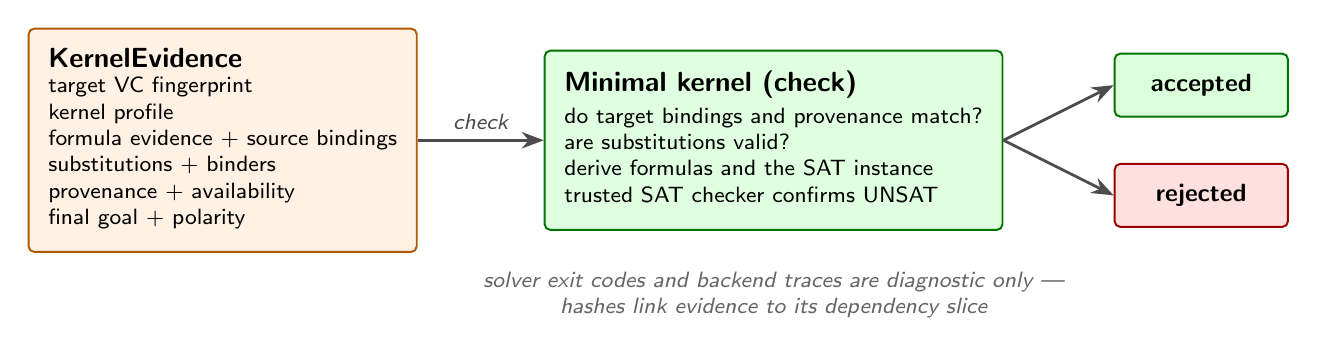
\begin{tikzpicture}[
  font=\sffamily,
  doc/.style={draw, rounded corners=2pt, align=left, line width=0.7pt,
              fill=orange!10, draw=orange!70!black, inner sep=2.5mm},
  kern/.style={draw, rounded corners=2pt, align=left, line width=0.7pt,
               fill=green!12, draw=green!45!black, inner sep=2.5mm},
  verdict/.style={draw, rounded corners=2pt, align=center, minimum width=22mm,
                  minimum height=8mm, line width=0.7pt, font=\sffamily\small\bfseries},
  flow/.style={-{Stealth[length=2.8mm]}, line width=1pt, black!70},
]
  \node[doc] (cert) {%
    \textbf{KernelEvidence}\\[1.5pt]
    \footnotesize
    \begin{tabular}{@{}l@{}}
      target VC fingerprint\\
      kernel profile\\
      formula evidence + source bindings\\
      substitutions + binders\\
      provenance + availability\\
      final goal + polarity
    \end{tabular}};

  \node[kern, right=16mm of cert] (kernel) {%
    \textbf{Minimal kernel (check)}\\[1.5pt]
    \footnotesize
    \begin{tabular}{@{}l@{}}
      do target bindings and provenance match?\\
      are substitutions valid?\\
      derive formulas and the SAT instance\\
      trusted SAT checker confirms UNSAT
    \end{tabular}};

  \node[verdict, fill=green!14, draw=green!45!black, anchor=west]
    (acc) at ([xshift=14mm,yshift=7mm]kernel.east) {accepted};
  \node[verdict, fill=red!12, draw=red!60!black, anchor=west]
    (rej) at ([xshift=14mm,yshift=-7mm]kernel.east) {rejected};

  \draw[flow] (cert) -- node[font=\sffamily\footnotesize\itshape, above] {check} (kernel);
  \draw[flow] (kernel.east) -- (acc.west);
  \draw[flow] (kernel.east) -- (rej.west);

  \node[font=\sffamily\footnotesize\itshape, text=black!60,
        below=4mm of kernel.south, align=center]
    {solver exit codes and backend traces are diagnostic only ---\\
     hashes link evidence to its dependency slice};
\end{tikzpicture}
\end{document}
